\documentclass[a4paper,11pt]{article}

\usepackage[utf8x]{inputenc}
\usepackage[T1]{fontenc}
\usepackage[francais]{babel}
\usepackage{amsmath,amssymb}
\usepackage{fullpage}
\usepackage{xspace}
\usepackage{verbatim}
\usepackage{graphicx}
\usepackage{listings}
\usepackage{mathrsfs}
\usepackage[usenames,dvipsnames]{color}
\usepackage{url}

\lstset{basicstyle=\small\tt,
  keywordstyle=\bfseries\color{Orchid},
  stringstyle=\it\color{Tan},
  commentstyle=\it\color{LimeGreen},
  showstringspaces=false}

\newtheorem{exo1}{Question}
\newtheorem{exo2}{Question}
\newtheorem{exo3}{Question}
\newtheorem{exo4}{Question}

\newcommand{\dx}{\,dx}
\newcommand{\ito}{,\dotsc,}
\newcommand{\R}{\mathbb{R}}
\newcommand{\C}{\mathbb{C}}
\newcommand{\N}{\mathbb{N}}
\newcommand{\Poly}[1]{\mathcal{P}_{#1}}
\newcommand{\abs}[1]{\left\lvert#1\right\rvert}
\newcommand{\norm}[1]{\left\lVert#1\right\rVert}
\newcommand{\pars}[1]{\left(#1\right)}
\newcommand{\bigpars}[1]{\bigl(#1\bigr)}
\newcommand{\set}[1]{\left\{#1\right\}}

\title{TP Statistiques : Compte-rendu}
\author{Michel Yoeung, Charles-Frédérick Amaudruz, Alexandre Berrada (ENSIMAG - 1A - Groupe 2)}
\date{Avril 2018}

\begin{document}

\maketitle

%======================================
\section{Première stratégie.}
%======================================

\begin{exo1} \ \\ \\
\[
  \forall i = 1,...,n, X_{i} = \left\{
                                  \begin{array}{ll}
                                    1 & \quad \mathrm{\text{si le $i^{eme}$ poisson est bagué}} \\
                                    0 & \quad \mathrm{sinon} \\
                                  \end{array}
                                \right.
\]
De plus, les résultats des pêches successives sont indépendants et la probabilité que le $i^{ème}$ poisson soit bagué est $p=\frac{n_{0}}{\theta}$. \ \\
Donc les $X_{i}$ sont indépendants et identiques (iid) car suivent tous une loi de Bernoulli de paramètre de succès $p=\frac{n_{0}}{\theta}$. \ \\
Soit $\theta=1000$ et $n_{0}=50$. On choisit $n=60$ pour notre simulation sur R. \ \\
On obtient l'échantillon de données suivant :
\begin{figure}[h]
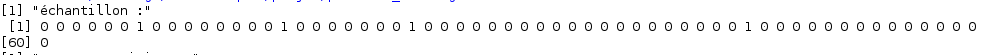
\includegraphics[scale=0.45]{images/Q1_1_donnees.png}
\end{figure} \ \\
On calcule ensuite sur R les moyennes et les variances (empiriques et théoriques) :
\begin{figure}[h]
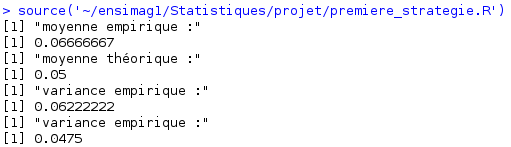
\includegraphics[scale=0.7]{images/Q1_1.png}
\end{figure} \ \\
On constate que pour ce jeu de données la moyenne empirique est assez proche de la moyenne théorique et de même pour les variances.
\end{exo1}

\begin{exo1} \ \\ \\
$T$ est une variable aléatoire qui compte le nombre de poissons bagués parmi les $n$ poissons pêchés donc $T=\sum_{i=1}^{n}X_{i}$ avec $X_{i}$ qui suit une loi de Bernoulli. \ \\
Donc $T$ suit une loi binomiale de paramètres $n$ et $p=\frac{n_{0}}{\theta}$. \ \\
On donne ainsi avec R $t$ le nombre de poissons pêchés sur notre échantillon de données :
\begin{figure}[h]
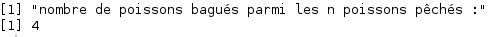
\includegraphics[scale=0.7]{images/Q1_2.png}
\end{figure} \ \\
\end{exo1}

\begin{exo1} \ \\ \\
Estimateur des moments : \ \\
Soit $\overline{X_{n}}$ la moyenne empirique, \ \\
\begin{equation}
\begin{aligned}
E[X] \simeq \overline{X_{n}} & \Rightarrow p \simeq \frac{1}{n}\sum_{i=1}^{n} x_{i} \ \\
& \Rightarrow \frac{n_{0}}{\theta} \simeq \frac{1}{n}\sum_{i=1}^{n} x_{i} \ \\
& \Rightarrow \theta \simeq \frac{n_{0}*n}{\sum_{i=1}^{n} x_{i}} \ \\
\end{aligned}
\end{equation} \ \\
Donc l'estimateur des moments (d'ordre 1) vaut $\tilde{\theta_{n}}=\frac{n_{0}*n}{\sum_{i=1}^{n} x_{i}}$. \ \\ \\
Estimateur de maximum de vraisemblance : \ \\ \\
\begin{equation}
\begin{aligned}
$ \mathscr{L}(X_{1}=x_{1},...,X_{n}=x_{n}, \theta) & = \prod_{i=1}^{n}\textsc{P}(X_{i}=x_{i}, \theta) \ \\
& = p^{\sum_{i=1}^{n} x_{i}}(1-p)^{n-\sum_{i=1}^{n} x_{i}} \ \\ 
& = (\frac{n_{0}}{\theta})^{\sum_{i=1}^{n}
x_{i}}(1-\frac{n_{0}}{\theta})^{n-\sum_{i=1}^{n} x_{i}} \ \\
\end{aligned}
\end{equation} \ \\
$\ln(\mathscr{L}(X_{1}=x_{1},...,X_{n}=x_{n}, \theta)) = (\sum_{i=1}^{n}x_{i})(\ln(n_{0})-\ln(\theta)})+(n-\sum_{i=1}^{n} x_{i})\ln(1-\frac{n_{0}}{\theta})$ \ \\ \\
En dérivant par rapport à $\theta$ : \ \\
\begin{equation}
\begin{aligned}
\frac{\partial\,\ln(\mathscr{L}(X_{1}=x_{1},...,X_{n}=x_{n}, \theta))}{\partial\,\theta} & = -(\sum_{i=1}^{n} x_{i})\frac{1}{\theta}+(n-\sum_{i=1}^{n} x_{i})\frac{\frac{n_{0}}{\theta^{2}}}{1-\frac{n_{0}}{\theta}} \ \\
& = -(\sum_{i=1}^{n} x_{i})\frac{1}{\theta}+(n-\sum_{i=1}^{n} x_{i})\frac{n_{0}}{\theta^{2}-\theta n_{0}} \ \\
& = 0 \Rightarrow \theta=\frac{n_{0}*n}{\sum_{i=1}^{n} x_{i}}
\end{aligned}
\end{equation} \ \\
Donc l'estimateur de maximum de vraisemblance vaut $\hat{\theta_{n}}=\frac{n_{0}*n}{\sum_{i=1}^{n} x_{i}}$. \ \\
Donc ces deux estimateurs sont confondus. \ \\
On calcule ainsi sur R la valeur de ces estimateurs sur notre échantillon de données : \ \\
\begin{figure}[h]
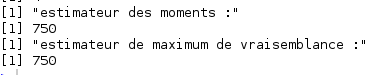
\includegraphics[scale=0.7]{images/Q1_3.png}
\end{figure} \ \\
Sur l'échantillon simulée, on observe un estimateur de $\theta$ qui vaut $750$ soit $25%$ de moins que la vraie valeur de $\theta$ pour al simulation ($1000$). \ \\
Cet estimateur n'est pas très précis.
\end{exo1}

\begin{exo1} \ \\ \\
intervalle de confiance exact de seuil $\alpha$ pour $\theta$ : \ \\
On a $p=\frac{n_{0}}{\theta} \Rightarrow \theta=\frac{n_{0}}{p}$ donc en estimant $p$ (avec la formule du cours), on obtient directement une estimation de $\theta$.
\begin{equation}
\begin{aligned}
\left{[}n_{0}(1+\frac{n-T}{T+1}f_{2(n-T),2(T+1),1-\frac{\alpha}{2}}),n_{0}(1+\frac{n-T+1}{T}f_{2(n-T+1),2T,\frac{\alpha}{2}})\right{]}
\end{aligned}
\end{equation} \ \\
avec $T=n\overline{X_{n}}=\sum_{i=1}^{n} x_{i}$ et $f_{\nu_{1},\nu_{2},\alpha} = F_{\mathscr{F}}^{-1}(1-\alpha,\nu_{1},\nu_{2})$, $F_{\mathscr{F}}^{-1}$ étant ici la fonction quantile de la loi de Fisher-Snedecor. \ \\
intervalle de confiance asymptotique de seuil $\alpha$ pour $\theta$ : \ \\
On obtient l'intervalle associée avec la même démarche que précédement.
\begin{equation}
\begin{aligned}
\left{[}\frac{n_{0}}{\overline{X_{n}}+u_{\alpha}\sqrt{\frac{\overline{X_{n}}(1-\overline{X_{n}})}{n}}},\frac{n_{0}}{\overline{X_{n}}-u_{\alpha}\sqrt{\frac{\overline{X_{n}}(1-\overline{X_{n}})}{n}}}\right{]}
\end{aligned}
\end{equation} \ \\
avec $u_{\alpha}=F_{\mathscr{N}}^{-1}(1-\frac{\alpha}{2})$, $F_{\mathscr{N}}^{-1}$ étant ici la fonction quantile de la loi normale. \ \\
On calcule ainsi ces intervalles de confiance (exacts puis asymptotiques) associés aux valeurs de nos paramètres fixés sur R pour les différentes valeurs de $\alpha$ spécifiées dans l'énoncé :
\begin{figure}[h]
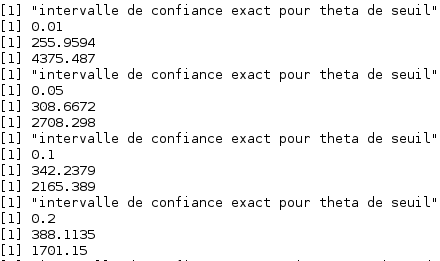
\includegraphics[scale=0.7]{images/Q1_4_exact.png}
\end{figure}
\begin{figure}[h]
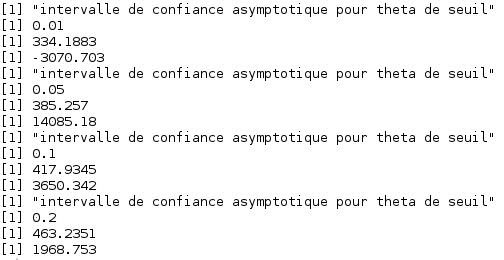
\includegraphics[scale=0.7]{images/Q1_4_asymp.png}
\end{figure} \ \\
On remarque que les intervalles exacts fournissent un encadrement plus précis de la vraie valeur de $\theta$ que les intervalles asymptotiques ce qui semble logique car les intervalles symptotiques sont plus efficaces pour un $n$ très grand, or ici on a fixé $n=60$ seulement.
\end{exo1}

\begin{exo1} \ \\ \\
$\textsc{P}(\hat{\theta_{n}}=+\infty) = \textsc{P}(\frac{n_{0}*n}{\sum_{i=1}^{n} x_{i}}=+\infty) = \textsc{P}(\sum_{i=1}^{n} x_{i}=0) = \textsc{P}(T=0) = (1-p)^n = (1-\frac{n_{0}}{\theta})^n$ \ \\
Cet estimateur n'est pas convergent. \ \\
$Biais(\hat{\theta_{n}}) = E[\hat{\theta_{n}}]-\theta$ \ \\
Comme $\hat{\theta_{n}}$ a une probabilité non nulle de valoir $+\infty$ alors $E[\hat{\theta_{n}}]=+\infty$ \Rightarrow $E[$\hat{\theta_{n}}$]-\theta = +\infty$ (car $\theta$ est une constante) \Rightarrow $Biais(\hat{\theta_{n}}) = +\infty$. \ \\
Donc on peut en déduire que le biais de cet estimateur vaut $+\infty$.
Sur notre échantillon de données, on peut calculer la probabilité $\textsc{P}(\hat{\theta_{n}}=+\infty)$ :
\begin{figure}[h]
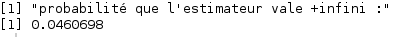
\includegraphics[scale=0.7]{images/Q1_5.png}
\end{figure} \ \\
\end{exo1}

\begin{exo1} \ \\ \\
\begin{equation}
\begin{aligned}
\textsc{P}(\hat{\theta_{n}}=+\infty) > \frac{1}{2} & \Rightarrow (1-\frac{n_{0}}{\theta})^{n} > \frac{1}{2} \ \\
& \Rightarrow n\ln(1-\frac{n_{0}}{\theta}) > \ln(\frac{1}{2}) \ \\
& \Rightarrow n < -\frac{\ln(2)}{\ln(1-\frac{n_{0}}{\theta})} \ \\
& \Rightarrow n \leq \lfloor-\frac{\ln(2)}{\ln(1-\frac{n_{0}}{\theta})}\rfloor
\end{aligned}
\end{equation} \ \\
Toujours avec notre échantillon de données, on calcule sur R cette valeur de n pour laquelle la probabilité $\textsc{P}(\hat{\theta_{n}}=+\infty)$ :
\begin{figure}[h]
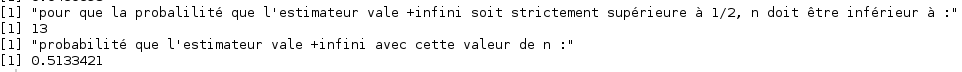
\includegraphics[scale=0.5]{images/Q1_6.png}
\end{figure} \ \\
\end{exo1}

\newpage

%======================================
\section{Deuxième stratégie.}
%======================================

\begin{exo2} \ \\ \\

\end{exo2}

\begin{exo2} \ \\ \\

\end{exo2}

\begin{exo2} \ \\ \\

\end{exo2}

\begin{exo2} \ \\ \\

\end{exo2}

\begin{exo2} \ \\ \\

\end{exo2}

\newpage

%======================================
\section{Application et comparaison des stratégies.}
%======================================

\begin{exo3} \ \\ \\

\end{exo3}

\begin{exo3} \ \\ \\

\end{exo3}

\begin{exo3} \ \\ \\

\end{exo3}

\begin{exo3} \ \\ \\

\end{exo3}

\newpage

%======================================
\section{Vérifications expérimentales à base de simulations.}
%======================================

\begin{exo4} \ \\ \\
On calcule R les différentes proportions d'appartenance de $\theta$ pour les intervalles de confiance établis en variant les paramètres.
\begin{figure}[h]
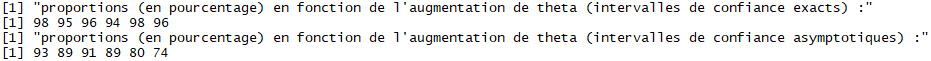
\includegraphics[scale=0.85]{images/Q4_1_theta.PNG}
\end{figure} \ \\
Lorsqu'on augmente $\theta$, on remarque que la proportion d'appartenance aux intervalles de $\theta$ diminue lorsqu'on choisit l'intervalle de confiance asymptotique. \ \\
En effet, lorsqu'on augmente $\theta$, la probabilité $p$ diminue donc l'intervalle asymptotique a une plus grande probabilité de se "tromper" car le nombre $n$ d'essais n'est pas grand.
\begin{figure}[h]
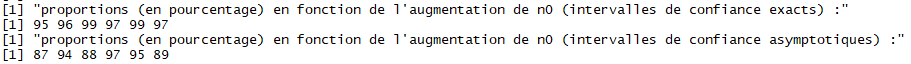
\includegraphics[scale=0.85]{images/Q4_1_n0.PNG}
\end{figure} \ \\
Lorsqu'on augmente $n_{0}$, on remarque que la proportion d'appartenance augmente très légèrement. \ \\
En effet, comme $n_{0}$ est proportionnel à $p$ et pour la même raison que précédemment, cela paraît cohérent.
\begin{figure}[h]
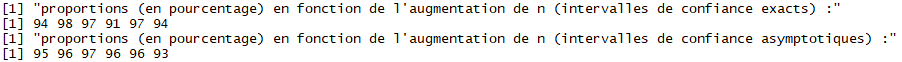
\includegraphics[scale=0.85]{images/Q4_1_n.PNG}
\end{figure} \ \\
Lorsqu'on augmente $n$, on ne constate pas de changement particulier, ce qui peut paraître incohérent car concernant l'intervalle asymptotique, ce dernier devrait être plus précis lorsque $n$ est grand.
\newpage
\begin{figure}[h]
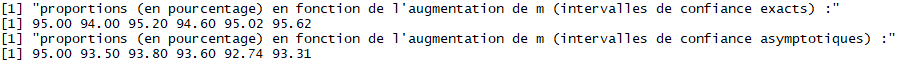
\includegraphics[scale=0.85]{images/Q4_1_m.PNG}
\end{figure} \ \\
Lorsqu'on augmente $m$, on constate une stabilisation au niveau des proportions donc de la précision des intervalles. \ \\
En effet, augmenter $m$ permet juste de rendre la simulation plus précise puisqu'on se base sur un plus grand nombre d'essais pour établir les proportions.
\begin{figure}[h]
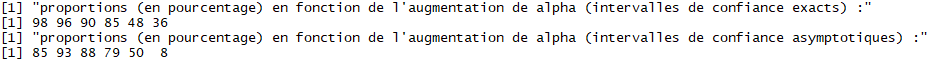
\includegraphics[scale=0.85]{images/Q4_1_alpha.PNG}
\end{figure} \ \\
Lorsqu'on augmente $\alpha$, quel que soit le type d'intervalle (exact ou asymptotique), il est cohérent que la proportion diminue car on baisse le niveau de confiance donc la précision de ces intervalles. \ \\
\end{exo4}

\begin{exo4} \ \\ \\
On simule $m=100$ échantillons de taille $n=5,10,100,1000,10000,100000$ de loi de Bernoulli, puis on compare les m moyennes empiriques avec les espérances (avec une erreur de $\epsilon=0.01$) pour illustrer la loi faible des grands nombres :
\begin{figure}[h]
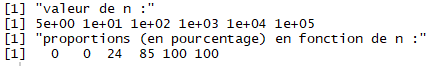
\includegraphics[scale=1.2]{images/Q4_2.PNG}
\end{figure} \ \\
Lorsque $n$ augmente, on remarque que l'écart entre la moyenne empirique et l'espérance diminue. A partir de $n=1000$ environ, on peut dire que la moyenne empirique peut être approximée par l'espérance. La loi faible des grands nombres est ainsi illustrée.
\end{exo4}

\begin{exo4} \ \\ \\
De la même manière que précédement, on va faire la même simulation avec $m=100$ et en faisant varier $n=5,30,50,100,1000,10000$, sauf qu'on va tracer les histogrammes (de même largeur en l'occurrence) des moyennes empiriques pour chaque valeur de $n$ ainsi que les graphes de probabilités associés pour la loi normale :
\newpage
\begin{figure}[h]
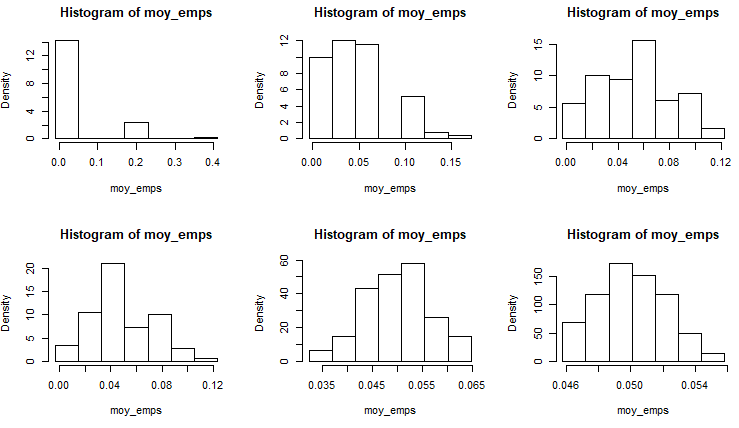
\includegraphics[scale=1]{images/Q4_3_histo.PNG}
\end{figure} \ \\
On remarque que la courbe associée à l'histogramme s'apparente à celle modélisant la fonction de densité de la loi normale à partir de $n=50$ environ.
\begin{figure}[h]
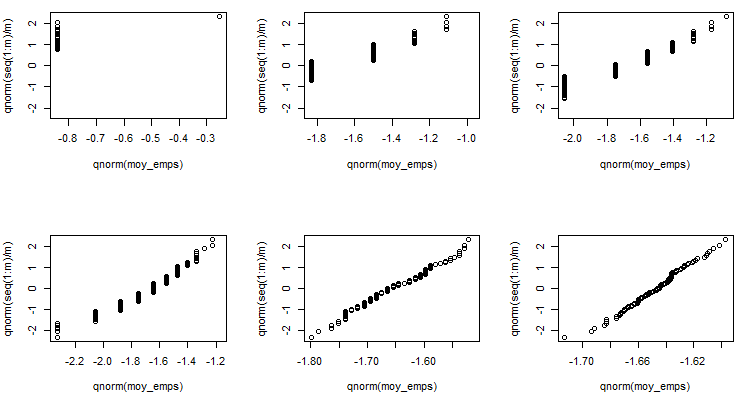
\includegraphics[scale=1]{images/Q4_3_proba.PNG}
\end{figure} \ \\
De même, en traçant les graphes de probabilité $(F_{\mathscr{N}}^{-1}(\overline{x_{i}}), $F_{\mathscr{N}}^{-1}(\frac{i}{m})$ avec $\overline{x_{i}} \forall i=1,...,n$ les moyennes empiriques de l'échantillon de données. On remarque de même que l'apparence d'une droite se forme à partir de $n=50$ ce qui confirme le fait qu'à partir de cette valeur de $n=50$ environ, la moyenne empirique des $x_{i}$ (iid suivant une loi de Bernoulli) suit une loi normale. Le théorème centrale limite est ainsi illustrée.
\end{exo4}

\end{document}
